Hasta este punto hemos introducido el problema y el contexto en el que ser circunscribe de manera generalista. En los siguientes apartados profundizaremos un poco más en el contexto del problema. Haremos un resumen del estado del arte de las áreas de conocimiento que vamos a trabajar. \medskip\par

\section{Imagen médica}
Situamos la primera imagen médica en 1895 con la imagen de rayos X de  Wilhelm Conrad Röntgen, pero no es hasta 1972 cuando encontraremos la primera imagen médica digitalizada: una tomografía computarizada de Godfrey Newbold Hounsfield. Paralelamente al desarrollo de la tecnología de los aparatos para la captación de imágenes hemos visto el desarrollo de las técnicas de la informática médica.\par
Encontramos en \cite{mantas2010recommendations}, una definición de lo que es la informática médica. Se trata del procesamientos sistemático de datos, información y conocimiento para la toma de decisiones óptima.\par
La medicina es un ámbito en que se puede aprovechar al máximo las nuevas posibilidades que nos ofrecen las tecnologías de la información. Es por esto que en los últimos 20 años hemos visto como ha florecido distintas líneas de investigación al rededor de la imagen médica.\par
Cuando hablamos de imagen médica nos referimos a un conjunto de técnicas y procesos para capturar imágenes del totales o parciales del cuerpo humano con propósitos cínicos.\cite{wiki:imgmedica}\par

En la literatura \cite{Muller20041,Maintz19981} podemos encontrar un repaso de los distintos dispositivos y tecnologías para captar imagen médica. Lo que es innegable es el gran impacto de la imagen médica en la práctica clínica. \medskip \par

Como afirmábamos en el apartado \ref{intro}, para hacer posible esta evolución son necesarios los estándares que permitan manipular las imágenes de manera óptima. Es precisamente por esto que se desarrolló el estándar de imagen médica DICOM. 
El acrónimo DICOM significa \textit{Imagen Digital y Comunicación en Medicina}. Por lo tanto no se trata únicamente del formato de la imagen sino que se diseñó para cubrir todas las necesidades vinculadas con la imagen médica. Necesidades como pueden ser: la compresión de imágenes, la comunicación, el almacenamiento, \ldots\par
Cada una de las necesidades específicas para el desarrollo de investigaciones y dispositivos relacionados con la imagen médica se recogen en el estándar y sus anexos que podemos encontrar en la web de la asociación Nacional de Fabricantes eléctricos (NEMA).\cite{nema}.\medskip\par

La literatura al respecto de la imagen médica en muy profusa. Por lo tanto, lo visto hasta el momento son únicamente los conceptos más básicos así como sus definiciones. La teoría sobre la imagen médica que hemos descrito forma parte de los cimientos sobre los que se sustenta este proyecto.\par

\section{Generación automática de código}
Otro de los pilares teóricos en los que se sustenta este proyecto es en la generación automática de código.\par
Cada una de las pruebas de imagen médica tiene asociado un informe DICOM-SR. Si nos planteáramos seguir un paradigma de programación diferente, necesitaríamos crear una aplicación Android para cada informe DICOM-SR. Aunque gran parte de este código fuera reutilizable, estaríamos desplazando el cuello de botella que ahora se encuentra en la captación de datos al desarrollo de aplicaciones.\par
Es por este motivo que optamos por la generación de código o traducción automática. Términos sinónimos en la literatura.\cite{802346}\medskip\par 
La generación automática de código es uno de los paradigmas de programación existentes y consiste en escribir programas que sean capaces de escribir el código fuente de otros programas basándose en modelos ontológicos.\par 
En nuestro caso los modelos ontológicos son las plantillas DICOM-SR. Para conseguir llevar a cabo esta tarea se dispone de un sistema de patrones que se instancian con los datos concretos, siguiendo unas reglas que son generalmente sencillas.\medskip\par
La generación automática de código es una de las líneas de investigación que más interés despierta en el ámbito de la ingeniería de software \cite{hinchey2005requirements}. Existe un buen número de razones para que esto sea así, a pesar de los desafíos que plantea este paradigma de programación. Entre los beneficios que ofrece la generación automática de código podemos enumerar los siguientes \cite{herrington2003code}:
\begin{itemize}
	\item \textit{Calidad}: El código generado mediante plantillas permite que la calidad sea consistente a lo largo de todo 	el software desarrollado y simplifica el proceso de aplicar parches que solucionen bugs. 
	\item \textit{Consistencia}: El estilo de programación mantiene una consistencia a lo largo de todo el software desarrolladoo.
	\item \textit{Más tiempo para el diseño del software y la arquitectura}: el análisis y desarrollo de la API en este paradigma es muy importante, por lo que se dedica más tiempo y recursos a captar los requisitos y crear la arquitectura. Estamos aprovechando el tiempo que de otro modo hubiéramos empleado en escribir manualmente el software.
	\item \textit{Abstracción}: la generación automática de código es independiente del lenguaje de programación, simplemente modificando el lenguaje de las plantillas podremos generar software en el lenguaje de programación que sea más conveniente. 
\end{itemize}
\medskip\par

La investigación actual tiene como gran reto el desarrollar modelos independientes del lenguaje y demostrar que el código que generan es computacionalmente equivalente al código generado por un desarrollador.\par
Sin embargo este enfoque queda fuera del alcance de nuestro proyecto. Lo que haremos es emplear las bases teóricas del paradigma de generación automática en nuestro desarrollo.\medskip\par
Existen diversas técnicas para generar código. Para este proyecto optamos por \textbf{generación parcial de clases}. La generación parcial de clases consiste en leer un fichero de texto con la información abstracta de las clases a generar, a continuación lee una serie de plantillas y con la información recogida de estas dos fuentes, generará el código necesario. Este código que hemos generado se integrará con el código escrito por ingenieros para formar la solución final.\par

En la figura \ref{fig:generacion} vemos como se aplica esta técnica de generación de código en nuestro ejemplo concreto. El sistema tendrá como entrada el informe médico de tipo DICOM-SR y una serie de plantillas, con esto generará el código necesario para que cuando lo integremos en la aplicación Android obtengamos una aplicación Android funcional específica para el informe de entrada. \par
\begin{figure}[ht]
\centering
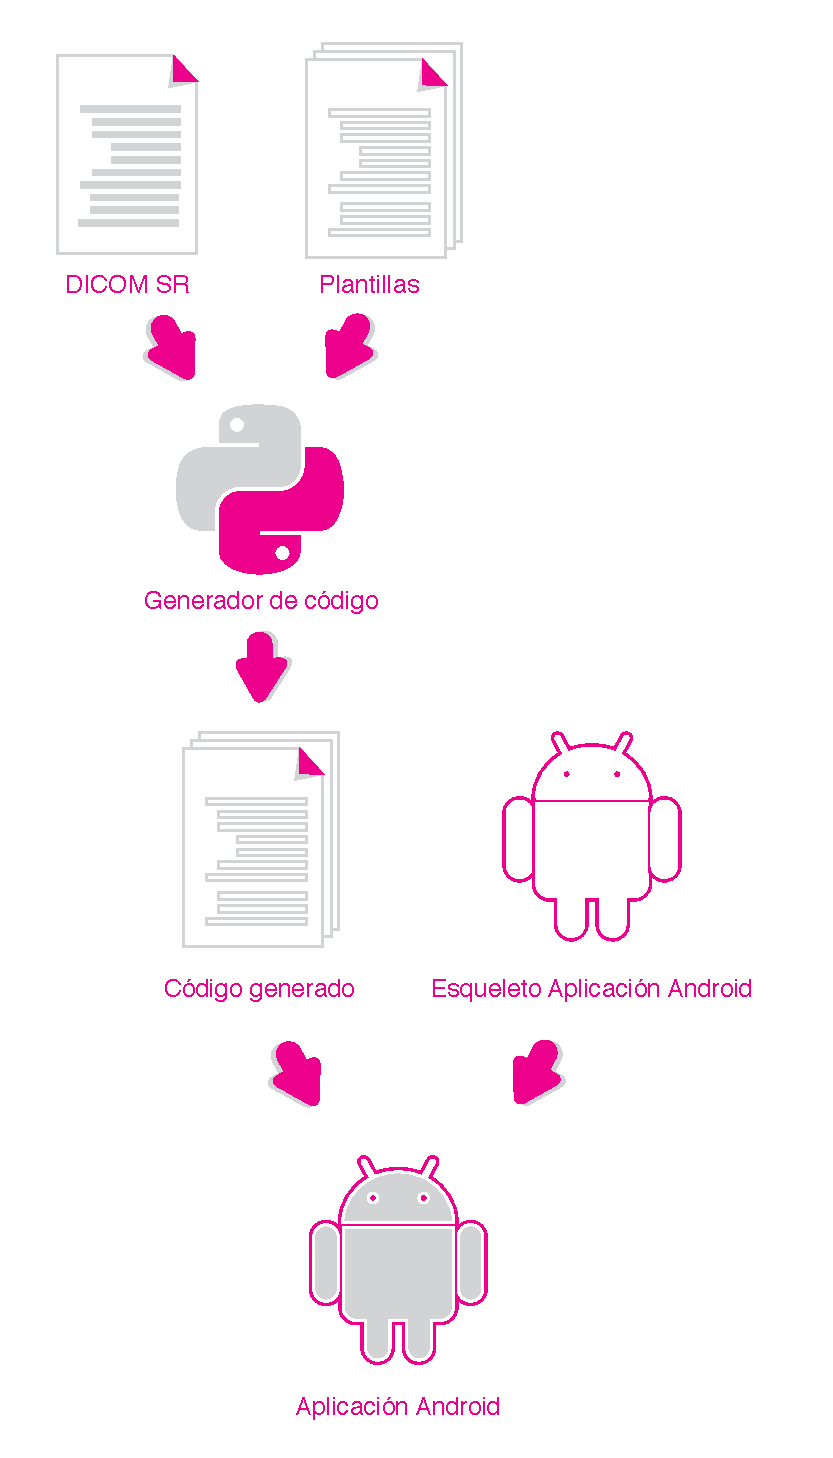
\includegraphics[scale=0.5]{./imgs/esquemas/generacion.pdf}
\caption{Generación parcial de clases}
\label{fig:generacion}
\end{figure}

\subsection{Desarrollo de software guiado por modelos}
El desarrollo de software guiado por modelos forma parte del paradigma de programación automática. De los paradigmas que descienden de la programación automática este es el que más se ajusta al trabajo que estamos presentando.\par
Consiste en desarrollar uno o varios modelos que representen el sistema y a partir de estos modelos se generará el software. Existen numerosas herramientas para definir modelos.\par
Según la literatura \cite{MDA} lo fundamental es que los modelos tengan las siguientes características:
\begin{itemize}
	\item Tan simples como sea posible (KISS).
	\item Canónico (DRY).
	\item Correcto nivel de abstracción.
	\item Separación de aspectos ( SoC ).
	\item Mantener modelos organizados y manejables.
	\item Independiente de la tecnología.
	\item Pragmáticos: sólo modelamos aquello que vayamos a emplear.
\end{itemize}
Podemos modelar todo o parte del sistema. Lo recomendable es que se modele aquello que varíe poco, con lo que el tiempo invertido en el modelado sea eficiente.\medskip \par

En nuestro caso el modelo viene determinado por el estándar soportado por los dispositivos PACs, es decir, utilizaremos los ficheros DICOM-SR como modelo para generar la aplicación.\par
Debido a las características del modelo, este proyecto no se adscribe dentro del desarrollo guiado por modelos tal y como se define en la literatura \cite{mdd}, pero si obviamos las características del modelo que vienen impuestas por los estándares médicos, seguimos la filosofía de este paradigma de programación, ya que a partir del modelo del sistema, el informe médico DICOM-SR, generamos el software con las características que el modelo define.\par


\section{Interacción persona-máquina y usabilidadad}
\chaptermark{Usabilidad}
Por último, antes de cerrar este capítulo nos falta hablar del tercer pilar que sustenta este proyecto: la interacción persona-máquina.\par
Como hemos discutido en la introducción \ref{intro}, uno de los problemas a los que nos enfrentamos a la hora de recoger informes médicos es que rellenar estos informes es una tarea pesada para los profesionales clínicos que deben invertir mucho tiempo en la captación de requisitos. La tecnología per se no soluciona este problema, sino que nos da herramientas para afrontarlo. Lo que es importante es que realicemos un diseño de las interfaces de usuario centrándonos en las necesidades de las personas que utilizarán las aplicaciones.\medskip\par
El término Interacción Persona-Máquina (\textit{\textbf{H}uman-\textbf{C}omputer \textbf{I}nteraction} en inglés) no se popularizó hasta la década de los 80, aunque podemos encontrar raíces similares en los estudios de ergonomía de principios del siglo XX \cite{dix2004human}. Pero es con el auge de la informática y diseño de sistemas cuando el estudio de la Interacción persona-máquina comienza a desarrollarse plenamente de manera autónoma. Con la aparición de los ordenadores personales todo el mundo se convirtió en un usuario potencial y era necesario encontrar formas de interactuar adecuadamente con este nuevo público. \par
La Interacción Persona-Máquina se encarga del diseño, implementación y validación de las interfaces de usuario. Es decir, se encarga de modelar cómo los usuarios se relacionan con las máquinas.\medskip\par
Al desarrollar un proyecto de este tipo corremos el peligro cuando estemos absortos en los detalles técnicos de olvidar la importancia del diseño. Un buen diseño debe centrarse en las personas, y tiene un tremendo impacto en las tareas que realizan a pesar de que el diseño será transparente para los usuarios.\par
En ámbitos que incluyan sistemas críticos como puede ser la medicina, los fallos en el diseño de las interacciones pueden tener un gran coste económico y personal. A pesar de que nuestro ámbito de aplicación no es crítico tenemos presente que la aceptación del sistema por parte de los usuarios es un punto clave para resolver el problema que nos planteamos en este proyecto.\medskip \par
Los puntos claves para conseguir un buen diseño de interfaces se basan en que todo el sistema sea consistente y en solicitar información al usuario final acerca de sus impresiones y sensaciones con el diseño.\par 
Respecto a la consistencia, esta es una ventaja propia de la generación automática de código ya que mientras seamos consistentes en el diseño de las plantillas la aplicación final tendrá una aspecto coherente.\par
Para conseguir la información acerca de la idoneidad del diseño, el procedimiento consiste en crear un diseño y evaluar la satisfacción por parte de los usuarios, con las respuestas que obtenemos de nuestro usuarios, que idealmente será un grupo diverso que represente a las personas que utilizarán la aplicación, cambiamos el diseño y solicitamos de nuevo una evaluación del diseño. Idealmente seguiríamos iterando en el diseño de este prototipo hasta llegar a un punto en el los usuarios estén satisfechos con el resultado. En la práctica se llega a una solución de compromiso entre el tiempo empleado en el diseño y la satisfacción de los usuarios.\par
En nuestro proyecto hemos integrado los ciclos de diseño y validación de la interfaces dentro del desarrollo de la aplicación. En la fases iniciales de diseño, creamos las interfaces que se fueron refinando durante el proceso, y empleamos la aplicación Android que nos serviría de esqueleto dónde integrar el código generado como prototipo para poder validar el diseño.\medskip \par
Finalizamos este apartado recalcando la importancia del diseño, muchas veces denostado, en la aceptación por parte de los usuarios de las soluciones software que les proponemos. 

